\documentclass{tietreport}

% Import images
\usepackage{graphicx}

% Packages added for this report (all part of TeX Live / Overleaf)
\usepackage{amsmath}
\usepackage{amssymb}
\usepackage{booktabs}
\usepackage{tabularx}
\usepackage{array}
\usepackage{tikz}
\usetikzlibrary{positioning, fit, arrows.meta, calc}
\usepackage{pgfplots}
\pgfplotsset{compat=1.18}
\usepackage{algorithm}
\usepackage{algpseudocode}
\usepackage{microtype}

\newcolumntype{Y}{>{\raggedright\arraybackslash}X}
\newcolumntype{P}[1]{>{\raggedright\arraybackslash}p{#1}}
\setlength{\emergencystretch}{3em}
\hypersetup{hidelinks}

% Bibliography configuration
\usepackage[
  date=year,
  style=alphabetic,
  backend=biber,
  sorting=nty,
  maxnames=5,
  minnames=3,
  maxalphanames=4,
  minalphanames=3,
  backref=true,
  doi=false,
  isbn=false,
  url=false,
  eprint=false
]{biblatex}
\addbibresource{references.bib}
\appto{\bibsetup}{\sloppy}

%% ==================================================
%% CUSTOMIZE THESE FIELDS FOR YOUR PROJECT
%% ==================================================

% Course/Lab header
% TODO: replace with the exact course code and title used by the department
\TitlePageHeader{%
  UCSXXX - Capstone Project%
}

% Main project title
\ProjectTitle{%
  IntelliSchedule%
}

% Subtitle or project description
\ProjectSubTitle{%
  Constraint-Based Timetable Generation, Validation and In-Semester
  Recovery for a Multi-Department University%
}

% Student information (up to 4 students)
% TODO: fill in roll numbers and names
\author{%
  \texttt{102XXXXXXX} Student Name One \\
  \texttt{102XXXXXXX} Student Name Two \\
  \texttt{102XXXXXXX} Student Name Three \\
  \texttt{102XXXXXXX} Student Name Four%
}

% Group number, degree, year, program
% TODO: group number and year
\TitlePageSubText{%
  Group: \texttt{XXXX} BE Third Year, CSE%
}

% Faculty advisor/guide name
% TODO: supervisor's name
\AdvisorName{%
  Dr. Faculty Member Name%
}

% Evaluation period and department info
\TitlePageFooterText{{%
    \large Mid-Semester Evaluation \\[0.2cm]
    \bfseries Computer Science and Engineering
    Department%
  } \\[0.15cm]
  Thapar Institute of Engineering and Technology,
  Patiala%
}

%% ==================================================

\begin{document}

% Generate title page
\maketitle

% ===== ABSTRACT =====

\chapter*{Abstract}
\addcontentsline{toc}{chapter}{Abstract}

Putting together the weekly timetable for a university of TIET's size is
a large constraint-satisfaction exercise. It is usually done by hand from a
master spreadsheet, and then repaired, again by hand, whenever a teacher is
away or a room is closed. This report describes IntelliSchedule, a web
platform we built to take on both halves of that job. A coordinator imports
the semester's master data. The system compiles it into a search problem,
screens it for infeasibility that can be detected up front, and produces a
clash-free draft with a two-phase engine: a backtracking search over bitset
occupancy masks, followed by simulated annealing on a weighted
soft-constraint penalty. Every candidate is re-checked by a separate
validator before it can be selected or published. After publication,
faculty can cancel classes, the system proposes make-up slots, and class
representatives can poll their sections on them. The platform runs as a
single Node.js/Express service with a React front end and a PostgreSQL store,
with role-based access for seven roles.

We evaluated the system on the repository's seeded instance (32 sections,
64 laboratory subgroups, 80 rooms, 736 weekly session-hours) and on a
synthetic family of instances up to 2,208 session-hours. Phase~A finds a
conflict-free timetable for the seeded instance in under 10\,ms (median
7.5\,ms), and the validator confirms zero hard violations. Phase~B lowers the
soft penalty by 2--6\%. In 19 of 30 runs, however, it also introduced a
cross-cohort clash, which the validator then caught. We traced this to a
single key that the annealer's fast feasibility check reads but never
writes. We also found that the search thrashes once there are fewer lecture
rooms than sections, and that its recursion can overflow the default call
stack from about 1,800 session-hours. The report ends with the changes these
findings point to.

% Table of contents (auto-generated from chapters)
\tableofcontents
\listoffigures
\listoftables

% ===== CHAPTER 1: INTRODUCTION =====

\chapter{Introduction}

\section{Background and Context}

An engineering timetable looks simple from a student's side: a grid of
five days and eight one-hour periods, with lunch from 12:00 to 13:00. The
work behind it is not simple. Every section has a fixed set of courses,
each with a weekly quota of lecture, tutorial and laboratory hours.
Laboratories are run for half-sections (subgroups such as CSE-A1 and
CSE-A2), which may sit in different labs at the same time, but never while
the whole section has a lecture. Lab sessions are two or three consecutive
periods in the same room. Rooms differ in capacity and equipment, and a
computer lab cannot stand in for a lecture hall or the other way round.
Teachers have periods they have blocked for research or administrative
duties, and an upper limit on weekly teaching hours. On top of these hard
rules sit the softer wishes that decide whether a timetable is pleasant or
miserable: no long idle gaps between classes, not too many classes in a row,
no running between buildings in a five-minute break, and the same course not
landing in the same period every day.

Finding an assignment that satisfies the hard rules is already difficult in
the formal sense. \textcite{even1976complexity} showed that timetabling
becomes NP-complete once teachers have restricted availability, and
\textcite{cooper1996complexity} showed that several other features of real
timetabling problems are each enough on their own to make construction
NP-complete. In practice most institutions, ours included, rely on an
experienced coordinator working from a master spreadsheet. The
repository we describe here ships with an example of such a workbook, a
Thapar master-setup file for a 500-student cohort, and the platform's import
format is built around it.

The second half of the problem gets much less attention. A timetable does
not stay fixed once it is published. Faculty travel to conferences, fall ill
or take on examination duty; a lab is closed for maintenance; a guest
lecture needs a hall. Each cancellation leaves the section short of contact
hours, and finding a make-up slot by hand means checking three calendars at
once: the section's, the teacher's and the rooms'. The research literature
calls the general version of this the \emph{minimal perturbation
problem}~\cite{muller2005minimal,phillips2017integer}: repair the timetable
after a change while disturbing as little of it as possible.

IntelliSchedule is our attempt to handle both problems in one system. It
takes the semester's master data, generates a clash-free draft, checks the
draft with an independent validator, routes it through review and approval,
and publishes it to role-specific portals for coordinators, heads of
department, administrators, faculty, class representatives and students.
After publication it supports cancellations, make-up proposals, student
polls on make-up slots, and versioned edits with an audit trail.

\subsection{Problem Statement}

Given the master data for one semester (working days and periods,
departments, courses with weekly hour quotas, faculty with availability and
load limits, rooms with type, capacity and equipment, sections with their
laboratory subgroups, and the allocation of each course component to a
teacher and a section or subgroup), the system must:

\begin{enumerate}
  \item produce a weekly timetable that satisfies every hard constraint
    listed in Section~\ref{sec:model}, or explain why none can exist;
  \item among feasible timetables, prefer ones with a low weighted penalty
    for gaps, long runs of classes, building changes and poor spreading of
    a course across the week;
  \item guarantee that no timetable reaches students unless an independent
    check has found zero hard violations and every required hour has been
    scheduled;
  \item let the right people, and only them, edit, approve and publish;
  \item after publication, propose clash-free make-up slots for a cancelled
    class without moving any other class.
\end{enumerate}

The scope is a weekly repeating timetable on one campus with one-hour
periods. Teacher assignment is an input, not a decision: the allocation
table already says who teaches what to whom. The solver decides only
\emph{when} and \emph{where}.

\section{Project Objectives}

We set the following objectives at the start of the semester. Each has a
measurable target, and Chapter~\ref{ch:results} reports against them.

\begin{enumerate}
  \item \textbf{O1 -- Conflict-free generation:} generate a timetable for the
    seeded TIET-scale instance (736 weekly session-hours) with zero hard
    violations, as judged by the independent validator, in under one second
    on a laptop.
  \item \textbf{O2 -- Soft-constraint optimisation:} reduce the weighted soft
    penalty of the feasible draft by a measurable margin without breaking
    any hard constraint.
  \item \textbf{O3 -- Publication gate:} block selection and publication of
    any timetable that has a hard violation or an unscheduled required hour.
  \item \textbf{O4 -- In-semester recovery:} for a cancelled lecture, return
    up to five clash-free make-up options in under 50\,ms.
  \item \textbf{O5 -- Role-based workflow:} support seven roles with
    server-enforced permissions and a Draft $\rightarrow$ Review
    $\rightarrow$ Approved $\rightarrow$ Published lifecycle with versioning
    and audit.
  \item \textbf{O6 -- Security baseline:} meet the OWASP-recommended controls
    relevant to a cookie-authenticated web application (password hashing,
    CSRF defence, rate limiting, uniform authentication errors), each
    covered by an automated test.
\end{enumerate}

All six were scheduled for completion before the end-semester evaluation.
O1, O3 and O4 are directly measurable; O2 is measured as percentage
reduction in penalty; O5 and O6 are judged by the automated suites in
Section~\ref{sec:testing}.

\section{Organisation of the Report}

Chapter~\ref{ch:lit} places the project within the timetabling literature.
Chapter~\ref{ch:method} describes the architecture, the formal problem
model and the implementation of each module. Chapter~\ref{ch:results}
reports the automated test results and our own measurements of the engine,
including several defects that the measurements exposed.
Chapter~\ref{ch:conclusion} summarises the findings and lists the work that
follows from them. Appendix~\ref{app:repro} explains how to reproduce every
number in the report.

% ===== CHAPTER 2: LITERATURE REVIEW =====

\chapter{Literature Review}
\label{ch:lit}

\section{Timetabling as a Family of Problems}

Educational timetabling is usually divided into three problems: school
(class--teacher) timetabling, university course timetabling, and
examination timetabling~\cite{schaerf1999survey,dewerra1985introduction}.
The second International Timetabling Competition (ITC-2007) split course
timetabling further into a \emph{post-enrolment} variant, where conflicts
come from individual student registrations, and a \emph{curriculum-based}
variant, where students are grouped into curricula that take the same set of
courses~\cite{mccollum2010itc}. \textcite{ceschia2023educational} give a
current overview of these formulations, their benchmark sets and the best
known results.

Our setting is closest to curriculum-based course timetabling: a section is
a curriculum, and two courses clash if they share a section or a teacher.
It differs from the standard formulation in four ways that matter for the
algorithm. Sections split into laboratory subgroups that may run in
parallel with each other but not with a whole-section lecture. Laboratories
occupy two or three contiguous periods in a single room. The lunch period is
reserved campus-wide. And teachers are fixed by the allocation table, so the
solver chooses only a time and a room for each session.

\section{Computational Complexity}

\textcite{dewerra1985introduction} gives the graph-theoretic view of the
basic class--teacher problem, where the task reduces to colouring the edges
of a bipartite multigraph and can be solved in polynomial time.
\textcite{even1976complexity} showed that adding teacher unavailability is
enough to make the problem NP-complete, and \textcite{cooper1996complexity}
extended the picture by identifying several independent features of real
problems, each sufficient on its own for NP-completeness. The practical
consequence is that no general algorithm is known that is guaranteed to be
fast on every instance. Real systems therefore rely on heuristics, on search
with good pruning, or on exact solvers applied to instances small or
structured enough to be tractable.

\section{Graph-Colouring Heuristics}

If each class meeting is a vertex, each pair of meetings that cannot share a
period is an edge, and each period is a colour, then a clash-free timetable
is a proper vertex colouring with no more colours than there are periods.
\textcite{welsh1967upper} made this connection explicit and gave the
largest-degree-first greedy ordering still taught today.
\textcite{brelaz1979new} introduced DSATUR, which at each step colours the
vertex whose neighbours already use the most distinct colours.
\textcite{carter1996examination} compared several such orderings, with
and without backtracking, on real examination data from a number of
universities; the data sets they published are still used as a benchmark.
\textcite{burke2007graph} went a step further and used tabu search to choose
\emph{which} ordering heuristic to apply at each stage, an early example of a
hyper-heuristic. \textcite{lewis2021guide} gives a modern book-length
treatment. These methods construct a feasible solution quickly but handle
rooms and soft preferences awkwardly, which is why they are usually the
first stage of a larger method rather than a complete one.

\section{Constraint Satisfaction and Exact Methods}

Seen as a constraint satisfaction problem, each session is a variable whose
domain is the set of (period, room) pairs, and backtracking search assigns
variables one at a time, undoing the most recent choice when it reaches a
dead end. \textcite{haralick1980increasing} established the
\emph{fail-first} principle: branch on the variable with the fewest
remaining values, and use forward checking to prune values that have become
impossible. \textcite{russell2021aima} describe the standard refinements:
minimum-remaining-values ordering, least-constraining-value ordering,
conflict-directed backjumping, and min-conflicts local search.

Exact optimisation is also viable for medium-sized instances.
\textcite{lach2012curriculum} decomposed curriculum-based timetabling into
an integer program over time slots followed by room assignment, and used it
to find new solutions, some of them proven optimal, for the Udine benchmark
instances.
\textcite{muller2009itc} combined constraint-based construction (iterative
forward search) with local search, and the resulting solver won two of the
three ITC-2007 tracks. That hybrid is the closest published relative of our
two-phase design.

\section{Metaheuristics}

Local search methods start from a complete timetable and improve it with
small moves. Simulated annealing~\cite{kirkpatrick1983optimization} accepts
a worsening move of size $\Delta$ with probability $e^{-\Delta/T}$, where the
temperature $T$ falls over time, so that the search can escape local minima
early and settle later. \textcite{abramson1991constructing} applied it to
school timetabling, including a parallel version.
\textcite{ceschia2012design} showed that a carefully engineered and
statistically tuned annealer is competitive with far more complex methods on
post-enrolment timetabling. Tabu search~\cite{glover1989tabu} forbids
recently reversed moves; \textcite{lu2010adaptive} adapted it to
curriculum-based timetabling with strong results.
\textcite{burke2017late} proposed late-acceptance hill climbing, which
needs only one parameter and is therefore attractive when there is no time
to tune a cooling schedule. The surveys by
\textcite{burke2002recent}, \textcite{lewis2008survey},
\textcite{pillay2014survey} and \textcite{babaei2015survey} agree on one
broad pattern: the most successful methods first build a feasible timetable
and then optimise soft constraints with moves that never leave the feasible
region. IntelliSchedule follows that pattern.

\section{Benchmarks}

ITC-2007~\cite{mccollum2010itc} gave the field shared problem definitions,
instance files and a public validator, and \textcite{bonutti2012benchmarking}
consolidated the curriculum-based formulations (UD1 to UD5), the data format
and the reference results. These benchmarks make it possible to say that one
algorithm is better than another, which is otherwise surprisingly hard,
because every institution's rules differ. Our instance is not in a standard
format, so the results in Chapter~\ref{ch:results} are internal
measurements, not benchmark comparisons. Exporting our model to the
curriculum-based format is listed as future work.

\section{Rescheduling and Minimal Perturbation}
\label{sec:mpp}

\textcite{muller2005minimal} defined the minimal perturbation problem for
course timetabling: after the input changes, find a new feasible timetable
that differs from the old one in as few assignments as possible. They
evaluated their approach on data from a large university timetabling
problem. \textcite{phillips2017integer} formulated the same problem as an
integer program and applied it to real university instances. IntelliSchedule's
recovery engine addresses a much narrower case. A single class is
cancelled, and we look for a make-up slot that requires moving
\emph{nothing} else. We then hand the choice to people: faculty accept or
decline, and the section can vote. The general problem, where a teacher's
long leave forces several classes to move at once, is outside what the
current engine attempts.

\section{Existing Systems}

UniTime~\cite{unitime}, which grew out of the work at Purdue described
above, is a mature open-source system for course and examination
timetabling and student scheduling, deployed as an institution-wide Java web
application. FET~\cite{fet} is a widely used free timetabling program that
runs as a desktop application. Both generate timetables well. Our reasons
for building rather than adopting were practical: we wanted a lightweight
deployment that one coordinator could run, an import path that matches the
spreadsheet our department already maintains, and post-publication
workflows (cancellation, make-up proposals, section polls) integrated with
the same data. We do not claim that IntelliSchedule generates better
timetables than either system.

\section{Summary and Positioning}

Table~\ref{tab:approaches} summarises the approaches above and how each one
is used in this project.

\begin{table}[htbp]
\centering
\small
\begin{tabularx}{\linewidth}{@{}P{3.3cm}YYP{2.8cm}@{}}
\toprule
\textbf{Approach} & \textbf{Strengths} & \textbf{Weaknesses} & \textbf{Use here} \\
\midrule
Graph-colouring construction\newline\cite{welsh1967upper,brelaz1979new,carter1996examination}
  & Fast; easy to explain; good starting point
  & Rooms and soft constraints bolted on
  & Ordering idea in Phase~A; DSATUR prototype in benchmark view \\
\addlinespace
Backtracking CSP with fail-first\newline\cite{haralick1980increasing,russell2021aima}
  & Feasible by construction when it succeeds
  & Exponential worst case; chronological backtracking can thrash
  & Phase~A \\
\addlinespace
Integer programming\newline\cite{lach2012curriculum,phillips2017integer}
  & Optimality bounds; natural for minimal perturbation
  & Modelling effort; solver size and licensing
  & Not used; candidate for recovery \\
\addlinespace
Simulated annealing\newline\cite{kirkpatrick1983optimization,abramson1991constructing,ceschia2012design}
  & Simple; strong when tuned
  & Needs fast incremental evaluation and tuning
  & Phase~B \\
\addlinespace
Tabu search, late acceptance\newline\cite{glover1989tabu,lu2010adaptive,burke2017late}
  & State of the art on curriculum benchmarks
  & More machinery to implement
  & Possible replacement for Phase~B \\
\addlinespace
Hybrids\newline\cite{muller2009itc}
  & Competition-winning
  & Complex to build and maintain
  & Design reference \\
\bottomrule
\end{tabularx}
\caption{Timetabling approaches from the literature and their role in IntelliSchedule}
\label{tab:approaches}
\end{table}

% ===== CHAPTER 3: METHODOLOGY & DESIGN =====

\chapter{Methodology and Design}
\label{ch:method}

\section{System Architecture}

\subsection{High-Level Design}
\label{sec:hld}

IntelliSchedule is a modular monolith. One Node.js~22 process running
Express~5 serves both the JSON API under \texttt{/api} and the built React
application, so the browser talks to a single origin and authentication can
use an \texttt{httpOnly} cookie instead of tokens held in JavaScript.
Figure~\ref{fig:architecture} shows the main components.

\begin{figure}[htbp]
  \centering
  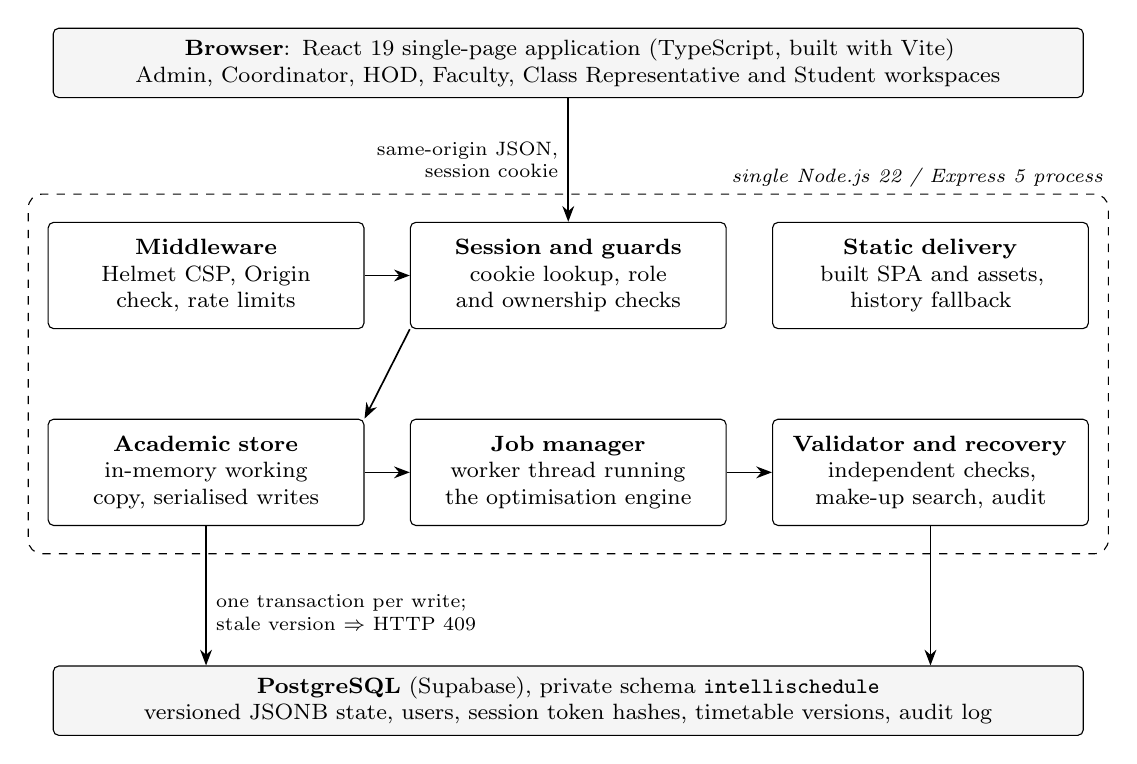
\begin{tikzpicture}[
      font=\footnotesize,
      box/.style={draw, rounded corners=2pt, align=center, inner sep=3pt,
                  text width=#1, minimum height=1.35cm},
      box/.default=3.8cm,
      wide/.style={draw, rounded corners=2pt, align=center, inner sep=4pt,
                   text width=12.8cm, fill=gray!8},
      arr/.style={-{Stealth[length=2mm]}, semithick},
    ]
    \node[wide] (spa) at (0,0)
      {\textbf{Browser}: React~19 single-page application (TypeScript, built with Vite)\\
       Admin, Coordinator, HOD, Faculty, Class Representative and Student workspaces};

    \node[box] (mw)     at (-4.6,-2.7) {\textbf{Middleware}\\ Helmet CSP, Origin\\ check, rate limits};
    \node[box] (auth)   at (0,-2.7)    {\textbf{Session and guards}\\ cookie lookup, role\\ and ownership checks};
    \node[box] (static) at (4.6,-2.7)  {\textbf{Static delivery}\\ built SPA and assets,\\ history fallback};

    \node[box] (store)  at (-4.6,-5.2) {\textbf{Academic store}\\ in-memory working\\ copy, serialised writes};
    \node[box] (engine) at (0,-5.2)    {\textbf{Job manager}\\ worker thread running\\ the optimisation engine};
    \node[box] (val)    at (4.6,-5.2)  {\textbf{Validator and recovery}\\ independent checks,\\ make-up search, audit};

    \node[draw, dashed, rounded corners=5pt, inner xsep=7pt, inner ysep=10pt,
          fit=(mw)(auth)(static)(store)(engine)(val)] (proc) {};
    \node[anchor=south east, font=\scriptsize\itshape, inner sep=2pt] at (proc.north east)
      {single Node.js~22 / Express~5 process};

    \node[wide] (db) at (0,-8.1)
      {\textbf{PostgreSQL} (Supabase), private schema \texttt{intellischedule}\\
       versioned JSONB state, users, session token hashes, timetable versions, audit log};

    \draw[arr] (spa.south) -- node[left, font=\scriptsize, align=right] {same-origin JSON,\\ session cookie} (auth.north);
    \draw[arr] (mw.east) -- (auth.west);
    \draw[arr] (auth.south west) -- (store.north east);
    \draw[arr] (store.east) -- (engine.west);
    \draw[arr] (engine.east) -- (val.west);
    \draw[arr] (store.south) -- node[right, pos=0.62, font=\scriptsize, align=left] {one transaction per write;\\ stale version $\Rightarrow$ HTTP 409} (store.south |- db.north);
    \draw[arr] (val.south) -- (val.south |- db.north);
  \end{tikzpicture}
  \caption{Runtime architecture of IntelliSchedule}
  \label{fig:architecture}
\end{figure}

The academic data and the live timetable are held in memory and written
through to PostgreSQL on every change. Each persisted document carries an
integer version. A write updates the row only if the version still matches
(\texttt{where key = \$1 and version = \$2}); if another process got there
first, the transaction rolls back, the request fails with HTTP~409 and the
server reloads its state. This is optimistic concurrency control in the sense
of \textcite{kung1981optimistic}. It prevents silent overwrites, but it also
means that only one instance may serve traffic, a constraint recorded in the
project's first architecture decision record.

One detail of the as-built system differs from the original design, and we
think it is worth stating plainly. The design documents describe four
normalised JSONB documents managed by a modular store. The running server
instead uses an older in-memory store and persists it as a single versioned
JSONB row, \texttt{legacy\_academic\_runtime}, with writes serialised inside
the process and committed before the HTTP response is sent. The modular
store exists in the code base but is not wired into the request path. Both
designs give the same guarantees for a single instance; neither scales out
without further work.

\subsection{Users, Roles and the Timetable Lifecycle}

The server recognises seven role codes, grouped as in
Table~\ref{tab:roles}. Roles are stored on the user record and checked on
every request. The browser never chooses a role; it only decides which
workspace to display. Ownership checks are applied on top of roles, so a
faculty member can cancel only their own classes and a class representative
can open polls only for their own section, following the role-based access
control model of \textcite{sandhu1996rbac}.

\begin{table}[htbp]
\centering
\small
\begin{tabularx}{\linewidth}{@{}P{3.2cm}P{3.0cm}Y@{}}
\toprule
\textbf{Role} & \textbf{Workspaces} & \textbf{Main permissions} \\
\midrule
Super Admin, College Admin & Admin, Coordinator & Everything a coordinator can do; final approval; user and session administration \\
Coordinator & Coordinator, Faculty & Master data, Excel import, generation, routine selection, manual edits, version restore, publication \\
Head of Department & HOD, Faculty & Department sign-off; add classes to the draft; cancel classes \\
Faculty & Faculty & Own timetable; mark unavailable periods; cancel own classes; accept or decline make-up options \\
Class Representative & Student, CR & Section timetable; open and close polls for own section; vote \\
Student & Student & Published section timetable; notifications; vote in section polls \\
\bottomrule
\end{tabularx}
\caption{Roles, workspaces and principal permissions}
\label{tab:roles}
\end{table}

A timetable moves through the states Draft, Review, Approved and Published.
Figure~\ref{fig:pipeline} shows the generation path and the two places where
the system can refuse to continue: the pre-generation audit, and the
independent validator.

\begin{figure}[htbp]
  \centering
  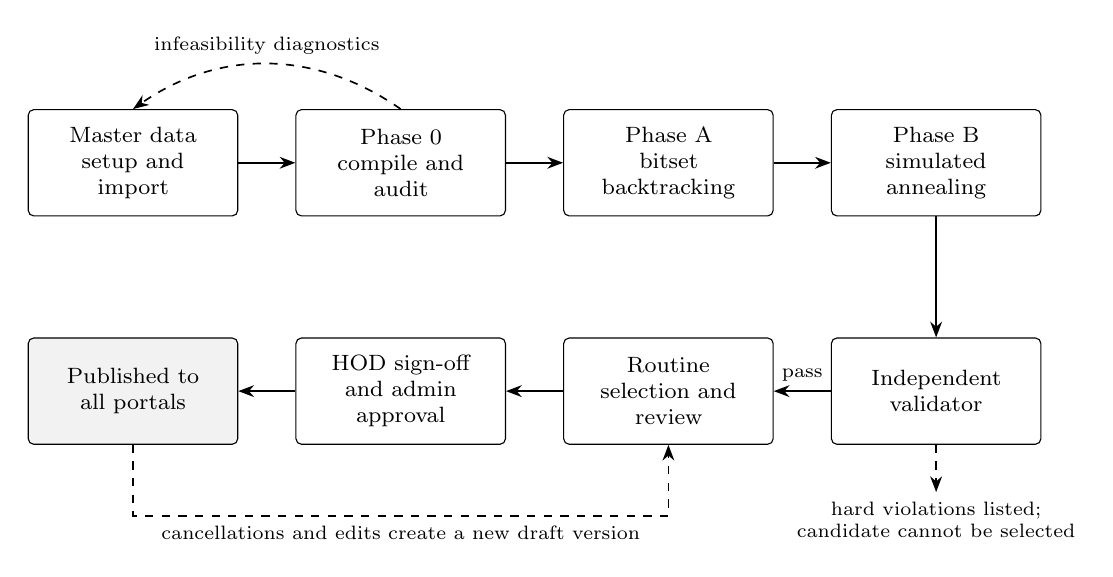
\begin{tikzpicture}[
      font=\footnotesize,
      stage/.style={draw, rounded corners=2pt, align=center, text width=2.45cm, minimum height=1.35cm, inner sep=3pt},
      arr/.style={-{Stealth[length=2mm]}, semithick},
      fail/.style={-{Stealth[length=2mm]}, semithick, dashed},
    ]
    \node[stage] (setup) at (0,0)    {Master data\\ setup and\\ import};
    \node[stage] (p0)    at (3.4,0)  {Phase 0\\ compile and\\ audit};
    \node[stage] (pa)    at (6.8,0)  {Phase A\\ bitset\\ backtracking};
    \node[stage] (pb)    at (10.2,0) {Phase B\\ simulated\\ annealing};

    \node[stage] (valid) at (10.2,-2.9) {Independent\\ validator};
    \node[stage] (sel)   at (6.8,-2.9)  {Routine\\ selection and\\ review};
    \node[stage] (appr)  at (3.4,-2.9)  {HOD sign-off\\ and admin\\ approval};
    \node[stage, fill=gray!10] (pub) at (0,-2.9) {Published to\\ all portals};

    \draw[arr] (setup) -- (p0);
    \draw[arr] (p0) -- (pa);
    \draw[arr] (pa) -- (pb);
    \draw[arr] (pb) -- (valid);
    \draw[arr] (valid) -- node[above, font=\scriptsize] {pass} (sel);
    \draw[arr] (sel) -- (appr);
    \draw[arr] (appr) -- (pub);

    \draw[fail] (p0.north) to[bend right=35] node[above, font=\scriptsize] {infeasibility diagnostics} (setup.north);
    \draw[fail] (valid.south) -- ++(0,-0.6) node[below, font=\scriptsize, align=center] {hard violations listed;\\ candidate cannot be selected};
    \draw[fail] (pub.south) -- ++(0,-0.9) coordinate (loopL) -- (loopL -| sel.south) node[pos=0.5, below, font=\scriptsize] {cancellations and edits create a new draft version} -- (sel.south);
  \end{tikzpicture}
  \caption{Generation, validation and publication pipeline}
  \label{fig:pipeline}
\end{figure}

\subsection{Technical Stack}

\begin{itemize}
  \item \textbf{Framework/Language:} TypeScript~5.7 on both sides. The client
    uses React~19, Vite~6 and Tailwind CSS~4; the server uses Node.js~22 with
    Express~5, run directly from TypeScript through \texttt{tsx} in
    development and bundled with esbuild for production.
  \item \textbf{Database:} PostgreSQL hosted on Supabase, reached through a
    direct connection string with the \texttt{pg} driver, inside a private
    schema with row-level security enabled and no policies, so the
    database's public REST roles see nothing. Development and tests use
    PGlite, an embedded PostgreSQL, so that no external service is needed.
  \item \textbf{Tools:} Git and GitHub with a pull-request workflow (127
    commits between 5~October and 17~November~2026); a GitHub Actions
    pipeline that type-checks, runs the unit/API, solver and security
    suites and builds the bundle; a multi-stage Docker image based on
    \texttt{node:22-alpine} with a readiness health check; deployment of the
    API as a single Render instance with the front end on Vercel, which
    proxies \texttt{/api/*} to the API host.
  \item \textbf{Libraries:} \texttt{bcryptjs} for password hashing,
    \texttt{helmet} for security headers, \texttt{zod} for request
    validation, \texttt{xlsx} (SheetJS) for parsing the master workbook in
    the browser, \texttt{nodemailer} for email, \texttt{google-auth-library}
    for Google sign-in, and \texttt{fast-check}, a property-based testing
    library in the QuickCheck tradition~\cite{claessen2000quickcheck}, in the
    test suites.
\end{itemize}

The code base is about 37,000 lines of TypeScript: 4,156 in the server entry
point, 5,911 in the scheduling and validation library, 5,530 in other server
modules, 17,300 in React components and contexts, and 3,900 in tests and
test scripts. The server exposes 95 HTTP routes.

\section{Problem Model}
\label{sec:model}

Let $\mathcal{D}$ be the working days and $\mathcal{P}$ the teaching periods
of a day, excluding lunch. The seeded configuration has $|\mathcal{D}| = 5$
and $|\mathcal{P}| = 7$, so the set of weekly slots
$\mathcal{T} = \mathcal{D} \times \mathcal{P}$ has 35 elements. Let
$\mathcal{R}$ be the rooms, $\mathcal{F}$ the faculty, $\mathcal{G}$ the
sections and $\mathcal{Q}_g$ the laboratory subgroups of section $g$. Each
allocation $a \in \mathcal{A}$ fixes a course $c(a)$, a teacher $f(a)$, a
section $g(a)$, optionally a subgroup $q(a)$, a weekly number of hours
$h_a$, and a session length $d_a$ (one period for lectures and tutorials,
two or three for laboratories). The binary decision variable
$x_{a,t,r} = 1$ means that one period of allocation $a$ is held in room $r$
at slot $t$.

\paragraph{Hard constraints.} The main hard constraints are:
\begin{align}
  \textstyle\sum_{t,r} x_{a,t,r} &= h_a
    && \forall a \in \mathcal{A} \tag{H1: completeness}\\
  \textstyle\sum_{a:\, f(a)=f}\sum_{r} x_{a,t,r} &\le 1
    && \forall f \in \mathcal{F},\ t \in \mathcal{T} \tag{H2: teacher clash}\\
  \textstyle\sum_{a} x_{a,t,r} &\le 1
    && \forall r \in \mathcal{R},\ t \in \mathcal{T} \tag{H3: room clash}\\
  w_{g,t} + s_{q,t} &\le 1
    && \forall g,\ q \in \mathcal{Q}_g \cup \{\varnothing\},\ t \tag{H4: cohort clash}
\end{align}
where $w_{g,t}$ counts whole-section periods of section $g$ at slot $t$ and
$s_{q,t}$ counts periods of subgroup $q$ (with $s_{\varnothing,t} = 0$, so
that H4 also forbids two whole-section classes at once). Two different
subgroups of the same section may therefore meet in parallel, but neither
may overlap a whole-section class. The remaining hard rules are stated in
words: a room must match the session type, hold the cohort and carry the
required equipment (H5); no session may use a teacher's protected period, a
teacher on leave or an unavailable room (H6); laboratory periods must form a
contiguous block of $d_a$ periods on one day in one room (H7); pinned
sessions stay where they were pinned (H8); a course may have at most one
lecture per day when its weekly hours do not exceed the number of days (H9);
and a teacher's weekly hours may not exceed their limit (H10).

Table~\ref{tab:hard} shows where each rule is enforced. The three columns
matter, because the results in Chapter~\ref{ch:results} turn on the
difference between them.

\begin{table}[htbp]
\centering
\small
\begin{tabularx}{\linewidth}{@{}P{3.3cm}YYY@{}}
\toprule
\textbf{Rule} & \textbf{Phase A (search)} & \textbf{Phase B (fast check)} & \textbf{Validator} \\
\midrule
H1 Completeness & By construction & Moves keep the count & Critical \\
H2 Teacher clash & Bitset test & Checked & Critical \\
H3 Room clash & Bitset test & Checked & Critical \\
H4 Cohort clash & Bitsets plus per-slot subgroup counters & Partly: a lecture placed after a subgroup session in the same slot is missed & Critical (three codes) \\
H5 Room suitability & Candidate-room filter & Checked & Critical \\
H6 Availability & Domain filter & Checked & Critical \\
H7 Lab contiguity & Atomic blocks & Labs never moved & Critical \\
H8 Pinned sessions & Pre-assigned & Pinned never moved & Critical \\
H9 One lecture a day & Hard rule & Not checked & Warning only \\
H10 Teacher weekly limit & Aggregate pre-check only & Not checked & Critical \\
\bottomrule
\end{tabularx}
\caption{Where each hard constraint is enforced}
\label{tab:hard}
\end{table}

\paragraph{Soft penalty.} The quality of a feasible timetable is measured by
a weighted penalty $P$, the sum of the terms in Table~\ref{tab:soft} minus a
bonus for sessions on a teacher's preferred days and periods. Three weight
profiles are built in. A coordinator can override any weight by storing a
constraint record with the matching code and a numeric parameter.

\begin{table}[htbp]
\centering
\small
\begin{tabularx}{\linewidth}{@{}Yccc@{}}
\toprule
\textbf{Penalty term (per occurrence)} & \textbf{Balanced} & \textbf{Student} & \textbf{Faculty} \\
\midrule
Idle period between two classes of a teacher on a day & 2 & 2 & 12 \\
Each period beyond three consecutive for a teacher & 3 & 3 & 6 \\
Idle period between two classes of a section on a day & 2 & 12 & 2 \\
Each period beyond three consecutive for a section & 4 & 8 & 4 \\
Each period beyond five in a section's day & 3 & 6 & 3 \\
Section day with a single period & 1 & 3 & 1 \\
Each extra meeting of the same course on one day & 5 & 10 & 5 \\
Back-to-back periods in different buildings & 5 & 10 & 5 \\
Each repeat of a course in the same period on another day & 3 & 3 & 3 \\
Room more than 40 seats larger than the section & 1 & 1 & 1 \\
Preferred day, preferred period (bonus, subtracted) & $-1$, $-1$ & $-1$, $-1$ & $-1$, $-1$ \\
\bottomrule
\end{tabularx}
\caption{Soft-constraint penalty terms and default weights for the three profiles}
\label{tab:soft}
\end{table}

The engine reports a \emph{health score}
$H = \min\bigl(100,\ \max(10,\ \mathrm{round}(100 - P))\bigr)$.
A second, unrelated health measure, used in the dashboards, combines faculty
load, student daily load, preference fit, room use, stability and syllabus
risk into a 0--100 figure, and is capped at 40 whenever a hard clash exists.
We keep the two apart in what follows, because the first one turns out to
saturate (Section~\ref{sec:health}).

\section{Implementation Details}

\subsection{Module 1: The Scheduling Engine}

The engine (\texttt{src/lib/optimizationEngine.ts}) runs in three phases.

\paragraph{Phase 0: compilation and infeasibility screening.} The master data
is converted into index-based arrays. Inactive teachers, teachers on leave
and unavailable rooms are dropped. For every allocation the compiler
computes the list of candidate rooms (right type, enough seats, all
required equipment), the list of feasible slots (excluding the teacher's
protected periods), and, for laboratories, every contiguous block of $d_a$
periods on a single day that avoids lunch. It then runs cheap necessary
checks, each of which produces a readable diagnostic instead of a silent
failure: an allocation with no suitable room; fewer feasible slots than
required hours; a section or a teacher whose total weekly hours exceed the
35 available slots; and total laboratory hours exceeding total lab-room
capacity. If any check fails, generation stops and the coordinator sees the
list.

\paragraph{Phase A: bitset backtracking.} Occupancy is held as one bit mask
per teacher, per room, per section and per subgroup, with bit $t$ set when
slot $t$ is taken. Checking whether teacher $f$ is free for a candidate block
$b$ is a single operation, $F_f \wedge b = 0$, and booking it is
$F_f \leftarrow F_f \vee b$. A whole-section lecture must also find no
subgroup session in the slot, which a small per-slot counter records. The
masks are JavaScript \texttt{BigInt} values, which comfortably hold the 35
bits needed. The project's micro-benchmark reports about 3.4\,ns per
\texttt{BigInt} AND on our test machine; it uses constant operands, so the
figure is best read as a lower bound.

Allocations are ordered once, before the search starts: laboratories first
(they have the tightest room and contiguity requirements), then by the ratio
of feasible slots to required hours, smallest first. This is a static form
of the fail-first rule~\cite{haralick1980increasing}. Algorithm~\ref{alg:phaseA}
gives the search. Values are tried in slot order for the first solution;
after that the value order is shuffled with the seeded generator so that
further candidates differ. Each room is chosen first-fit from the candidate
list. Lectures of one course are kept on different days when the weekly
hours allow it, and never in adjacent periods otherwise.

\begin{algorithm}[htbp]
\caption{Phase A: depth-first search over allocations (simplified)}
\label{alg:phaseA}
\begin{algorithmic}[1]
\Require allocations $A$ ordered labs first, then by $|D_a| / h_a$ ascending
\Function{Solve}{$i$}
  \If{time budget exhausted}
    \State \Return \textsc{false}
  \EndIf
  \If{$i = |A|$}
    \State record a candidate; \Return \textsc{true} if enough candidates
  \EndIf
  \State $a \gets A[i]$
  \If{$a$ already has $h_a$ hours}
    \State \Return \Call{Solve}{$i+1$}
  \EndIf
  \ForAll{values $v$ of $a$} \Comment{a slot, or a contiguous block for labs}
    \State $b \gets$ bit mask of $v$
    \If{$F_{f(a)} \wedge b \ne 0$ \textbf{or} the cohort is busy in $b$}
      \State \textbf{continue}
    \EndIf
    \State $r \gets$ first room in $R_a$ with $B_r \wedge b = 0$
    \If{no such room}
      \State \textbf{continue}
    \EndIf
    \State set $b$ in $F_{f(a)}$, $B_r$ and the cohort masks; record $(v, r)$
    \If{\Call{Solve}{$i'$}} \Comment{$i' = i+1$ once $a$ is complete, else $i$}
      \State \Return \textsc{true}
    \EndIf
    \State clear $b$ from the same masks; remove the record
  \EndFor
  \State \Return \textsc{false}
\EndFunction
\end{algorithmic}
\end{algorithm}

Note that the recursion descends one level for every placement, not for
every allocation. A three-hour lecture adds three frames. The depth of the
recursion is therefore close to the number of weekly session-hours, which
becomes important in Section~\ref{sec:stack}.

\paragraph{Phase B: simulated annealing.} If a feasible candidate exists and
the budget mode is not \textsc{fast}, each candidate is improved by the
annealer in Algorithm~\ref{alg:phaseB}. Three neighbourhoods are used:
swapping the slot and room of two sessions (45\% of proposals), moving one
session to a random slot and lecture room (35\%), and changing only the room
(20\%). Laboratory and pinned sessions are never moved. A proposal is first
screened by a fast hard-constraint check; if it passes, the full penalty is
recomputed and the move is accepted by the Metropolis rule. The schedule
starts at $T_0 = 10$, cools geometrically by $\alpha = 0.98$ per evaluated
move down to $T_{\min} = 0.01$, and reheats to $T = 6$ after 25 consecutive
rejections. The loop stops after 300 proposals or when the time budget runs
out, whichever comes first.

\begin{algorithm}[htbp]
\caption{Phase B: simulated annealing over feasible timetables}
\label{alg:phaseB}
\begin{algorithmic}[1]
\Require feasible timetable $X$; penalty $P$; $T_0 = 10$, $\alpha = 0.98$, $T_{\min} = 0.01$
\State $X^{*} \gets X$; $T \gets T_0$; $s \gets 0$
\For{$k \gets 1$ \textbf{to} $300$}
  \State draw $u \sim U(0,1)$
  \If{$u < 0.45$}
    \State $Y \gets$ swap slot and room of two movable sessions
  \ElsIf{$u < 0.80$}
    \State $Y \gets$ move one session to a random slot and lecture room
  \Else
    \State $Y \gets$ give one session a different lecture room
  \EndIf
  \If{$Y$ fails the fast hard-constraint check}
    \State \textbf{continue}
  \EndIf
  \State $\Delta \gets P(Y) - P(X)$
  \If{$\Delta < 0$ \textbf{or} $e^{-\Delta/T} > U(0,1)$}
    \State $X \gets Y$; $s \gets 0$
    \If{$P(X) < P(X^{*})$}
      \State $X^{*} \gets X$
    \EndIf
  \Else
    \State $s \gets s + 1$
  \EndIf
  \State $T \gets \max(T_{\min}, \alpha T)$
  \If{$s \ge 25$}
    \State $T \gets 6$; $s \gets 0$ \Comment{reheat}
  \EndIf
\EndFor
\State \Return $X^{*}$
\end{algorithmic}
\end{algorithm}

\paragraph{Seeding and determinism.} Randomness comes from a 32-bit xorshift
generator~\cite{marsaglia2003xorshift} seeded from the request (default
1337). Our project's solver suite runs the engine ten times with the same
seed and checks that the JSON output is byte-for-byte identical; it is. One
qualification applies: Phase~B is cut off by wall-clock time as well as by
its iteration cap, so on a slow machine, or under a small budget, two runs
with the same seed can stop at different points.

\paragraph{Running the engine without blocking the server.} Generation can
be requested synchronously or as a job. The job API
(\texttt{POST /api/timetable/jobs}) returns HTTP~202 immediately and runs the
engine in a Node.js worker thread, so the single server process keeps
answering other requests; the client polls the job and asks for the result
to be applied. The synchronous path generates two \emph{routines} by default,
one with the student-focused profile (seed 1337) and one with the
faculty-focused profile (seed 9999), validates both, and presents them side
by side with their metrics so the coordinator can choose.

\subsection{Module 2: Independent Validation and the Publication Gate}

The validator (\texttt{src/lib/independentValidator.ts}) shares no code with
the engine. It re-derives every clash from the session list alone, using hash
maps keyed by teacher, room and section per slot, and reports violations
under 24 codes, each marked \textsc{critical} or \textsc{warning}, with the
sessions involved, a message and a suggested fix. A timetable is
\emph{valid} when it has no critical violation, and \emph{publishable} when
it is valid and every required hour is scheduled.

The validator is consulted at four points: when routines are generated (each
one is labelled valid or not, with its blocking reasons), when a coordinator
selects a routine (refused if it has hard violations), when a job's result
is applied (HTTP~422 if not publishable), and when anyone tries to publish
(HTTP~422 with the count of conflicts and unscheduled hours). Manual moves
and swaps are checked by dedicated functions before they are applied. We
designed it this way on the principle that a solver should not be trusted
to mark its own homework. Chapter~\ref{ch:results} shows that the principle
paid off.

\subsection{Module 3: Disruption Recovery}

When a faculty member cancels a class, the server marks the session
cancelled, notifies the affected section and creates a make-up task. The
recovery search (\texttt{findSelfHealing}\allowbreak\texttt{RecoverySlots})
scans every teaching
slot of the week except the cancelled one and keeps a slot when three things
hold: no active session of the section (whole class or any subgroup) is
running, the teacher is free, and at least one available room of the right
type and size is free. Among the free rooms it picks the smallest that fits.
A slot freed by \emph{another} teacher's cancellation is recognised and
labelled as a cross-cancellation opportunity. Each surviving slot is scored
as
\begin{equation}
  S = 0.25\,T_{\mathrm{avail}} + 0.25\,S_{\mathrm{avail}} + 0.15\,R_{\mathrm{suit}}
    + 0.15\,U + 0.10\,P_{\mathrm{pref}} + 0.10\,B_{\mathrm{stab}},
\end{equation}
where each factor is on a 0--100 scale: teacher availability (80 if the slot
is one of the teacher's protected periods, otherwise 100), student
availability (98 for a cross-cancellation, otherwise 95), room suitability,
syllabus urgency (derived from the task's priority), preference (95 for the
first four periods, 85 later, 60 on Saturday) and stability. The five best
slots are returned. No other session is moved, so in the language of
Section~\ref{sec:mpp} the perturbation is zero by construction.

Two supporting features sit around this search. A substitute-teacher
ranking lists qualified colleagues who are free at the cancelled time,
penalising protected periods and teachers already at their load limit. A
what-if simulator lets a coordinator see which classes, teachers and
sections a room closure or a teacher's leave would affect before committing
to it. Staff can open polls in any section and class representatives in
their own, typically on candidate make-up slots; students vote and can change
their vote while the poll is open.

\subsection{Module 4: Academic Setup and Data Import}

All master data can be edited through the Academic Setup hub, which has tabs
for departments, programmes, courses, faculty, rooms, groups and subgroups,
students, and course allocations. For bulk entry the coordinator uploads the
master workbook. It is parsed in the browser with SheetJS and sent to the
server as JSON rows (\texttt{POST /api/academic/import}), where it is
committed in one step. A pre-generation audit then reports, before any search
starts, the problems that would make generation fail: no working days, no
allocations, missing rooms for a course's requirements, and the Phase~0
capacity checks.

\subsection{Module 5: Authentication, Authorisation and Security}

The controls follow the OWASP guidance for cookie-authenticated
applications~\cite{owasp2021top10,owaspcsrf}:

\begin{itemize}
  \item \textbf{Sessions.} A random session token is sent only as an
    \texttt{httpOnly}, \texttt{SameSite=Lax} cookie (secure in production)
    with a 24-hour lifetime. The server stores a hash of the token, never the
    token itself, and logout revokes it.
  \item \textbf{Passwords.} Passwords are hashed with bcrypt at cost
    12~\cite{provos1999future}. Hashes in older formats (scrypt, salted
    SHA-256) are still accepted and are transparently re-hashed with bcrypt
    at the next successful login. The policy requires 12 to 128 characters
    with upper case, lower case, a digit and a symbol.
  \item \textbf{Cross-site request forgery.} Every state-changing
    \texttt{/api} request whose \texttt{Origin} header is neither the
    server's own host nor on an allow-list is rejected with
    \texttt{403 CSRF\_ORIGIN\_DENIED}. Together with \texttt{SameSite} cookies
    this covers the cases in the OWASP cheat sheet.
  \item \textbf{Headers.} Helmet sets a content security policy that allows
    scripts only from the same origin, forbids framing and restricts
    \texttt{connect-src}. API responses carry \texttt{Cache-Control: no-store}.
  \item \textbf{Abuse limits.} Fixed-window rate limits apply per IP address
    and per account: for example 30 login attempts per minute per IP and 15
    per account, 5 password-reset requests per minute per IP, and 2 solver
    benchmark runs per minute per user.
  \item \textbf{Enumeration.} Unknown accounts and wrong passwords return the
    same HTTP~401 message, and duplicate registrations return the same
    generic HTTP~201 as new ones, so neither endpoint reveals whether an
    address is registered.
  \item \textbf{Registration.} Self-registration is limited to institutional
    email domains, and any role sent in the request body is ignored;
    self-registered accounts become students.
\end{itemize}

\subsection{Front End and Deployment}

The client is organised by workspace: about thirty views, including the
timetable grid with move, swap and lock actions, routine comparison, the Academic
Setup hub, a solver benchmark page, the what-if simulator, the recovery
engine view, and the student, faculty, class-representative, HOD and admin
portals. Every change goes through the API and the interface updates only
after the server confirms the write. The bootstrap data is refreshed every
ten seconds so that a cancellation made by a teacher appears on students'
screens without a reload. Timetables can be exported as CSV, as a recurring
iCalendar (ICS) feed, or printed to PDF.

% ===== CHAPTER 4: RESULTS & EVALUATION =====

\chapter{Results and Evaluation}
\label{ch:results}

\section{Testing Methodology}
\label{sec:testing}

We tested at four levels, using the project's own suites and an additional
measurement harness of our own:

\begin{itemize}
  \item \textbf{Unit Testing:} 24 tests run with the Node.js test runner,
    covering the engine, password hashing and migration, one-time tokens,
    persistent state, CSRF and security headers, timing-based account
    enumeration, and a pre-registration account-takeover scenario.
  \item \textbf{Integration Testing:} an end-to-end audit script starts the
    server on a local port and exercises the HTTP API as different users (54
    assertions covering health checks, authentication flows, Google sign-in
    error handling, timetable generation, master-data audits and relational
    integrity of the generated timetable). A separate adversarial suite (20
    attacks) checks unauthenticated access, forged tokens, privilege
    escalation, role injection, OAuth state tampering and password-reset
    abuse.
  \item \textbf{Performance Testing:} the project's solver suite (latency at
    four sizes, determinism, concurrency, infeasibility detection, lab
    blocks, pinned sessions, subgroups) and our own harness, which drives the
    engine, validator and recovery search directly with fixed seeds and
    reports medians and 95th percentiles. Our harness imports the project's
    modules unchanged; it does not modify any of them.
  \item \textbf{User Testing:} we have not yet run a structured study with
    coordinators, faculty or students. The interface has been exercised
    through demo accounts for each role during development, which is not the
    same thing, and a small usability study is planned for the second half
    of the semester (Section~\ref{sec:future}).
\end{itemize}

All measurements were taken on commit \texttt{cfca8da} (17~November~2026)
on a laptop with a 13th-generation Intel Core i5-1340P, 16\,GB of memory,
Windows~11 and Node.js~22.23.5. Timings are wall-clock milliseconds measured
inside the process with \texttt{performance.now()}.

\section{Performance Metrics}

\subsection{Automated Test Outcomes}

Table~\ref{tab:tests} summarises the automated suites. Type-checking is
clean, the unit tests all pass, and three assertions fail across the HTTP
suites. We looked at each failure before deciding how to report it.

\begin{table}[htbp]
\centering
\small
\begin{tabularx}{\linewidth}{@{}lccY@{}}
\toprule
\textbf{Suite} & \textbf{Passed} & \textbf{Failed} & \textbf{Notes} \\
\midrule
TypeScript (\texttt{tsc --noEmit}) & -- & 0 errors & \\
Unit tests & 24 & 0 & 5.9\,s \\
End-to-end API audit & 53 & 1 & Expects pre-verification login to fail; behaviour changed in commit \texttt{cfca8da} \\
Adversarial security suite & 18 & 2 & Coordinator publish allowed by documented policy; admin publish refused by the validator gate \\
Project solver suite & all sections & -- & Some reported metrics need care (Section~\ref{sec:minor}) \\
\bottomrule
\end{tabularx}
\caption{Results of the automated test suites on commit \texttt{cfca8da}}
\label{tab:tests}
\end{table}

The end-to-end failure is test drift, not a regression. The latest commit
deliberately allows a newly registered account to sign in before verifying
its email, because the production deployment had no mail provider configured
and verification links were never delivered. That commit updated two unit
tests but not the audit script. Of the two security-suite failures, the
first expects a coordinator's publish request to be refused, whereas
coordinator publication was added on purpose and is documented in the
project's permission matrix. The second is more interesting: the
administrator's publish request was refused with HTTP~422 by the
publication gate, because the draft that the coordinator had generated a
moment earlier in the same test run contained a hard clash. That clash is
the defect described in Section~\ref{sec:leak}.

\subsection{Generation on the Seeded Instance}

Table~\ref{tab:dataset} describes the instance that ships with the
repository. It is generated deterministically and stands in for one
semester across five departments.

\begin{table}[htbp]
\centering
\small
\begin{tabular}{@{}lr@{\quad}lr@{}}
\toprule
\textbf{Item} & \textbf{Value} & \textbf{Item} & \textbf{Value} \\
\midrule
Working days & 5 & Sections & 32 \\
Periods per day & 7 & Lab subgroups & 64 \\
Weekly slots & 35 & Students & 1,280 \\
Lecture/seminar rooms & 38/12 & Courses & 80 \\
Computer/hardware labs & 20/10 & Allocations (lect./lab) & 160/128 \\
Faculty (with allocations) & 500 (224) & Session-hours (lect./lab) & 480/256 \\
\bottomrule
\end{tabular}
\caption{Characteristics of the seeded instance}
\label{tab:dataset}
\end{table}

Every section has 15 lecture hours and 8 subgroup laboratory hours a week.
No teacher has more than five hours of allocations, and no teacher has a
protected period. We return to what this implies in
Section~\ref{sec:seeded}.

We ran the engine ten times per weight profile with ten different seeds,
first in \textsc{fast} mode (Phase~A only) and then in \textsc{balanced} mode
(Phases~A and~B, 800\,ms budget), and passed every result to the
independent validator. Table~\ref{tab:phaseab} gives the results.

\begin{table}[htbp]
\centering
\small
\begin{tabularx}{\linewidth}{@{}Yccc@{}}
\toprule
 & \textbf{Balanced} & \textbf{Student} & \textbf{Faculty} \\
\midrule
Penalty after Phase A & 3,213 & 5,926 & 2,819 \\
Penalty after Phase B (mean $\pm$ s.d.) & 3,022.7 $\pm$ 30.2 & 5,796.5 $\pm$ 54.1 & 2,670.3 $\pm$ 32.6 \\
Reduction, mean (min--max) & 5.9\% (5.0--7.5) & 2.2\% (0.7--3.7) & 5.3\% (3.1--6.7) \\
Health score before / after & 10 / 10 & 10 / 10 & 10 / 10 \\
Phase A time, median (ms) & 7.5 & 76.3 & 82.1 \\
Phase B time, median (ms) & 255.7 & 293.1 & 299.2 \\
Phase A backtracks (max) & 0 & 0 & 0 \\
Hard violations after Phase A & 0 & 0 & 0 \\
Hard violations after Phase B, max & 4 & 3 & 2 \\
\bottomrule
\end{tabularx}
\caption{Phase A and Phase B on the seeded instance (10 seeds per profile)}
\label{tab:phaseab}
\end{table}

Four things stand out. Phase~A solves the instance without a single
backtrack, and its output is identical for every seed, because the seed is
used only after the first solution. Phase~B reduces the penalty by a few
per cent, and a larger budget does not help: \textsc{maximum} mode with a
2\,s budget gave exactly the same penalty as \textsc{balanced} in 10 of 10
runs, because the 300-proposal cap is reached first. The health score is 10
before and after, the floor of its range. And the annealer's output
sometimes fails validation, which Phase~A's never does.
Figure~\ref{fig:penalty} breaks the balanced-profile penalty into its terms.

\begin{figure}[htbp]
\centering
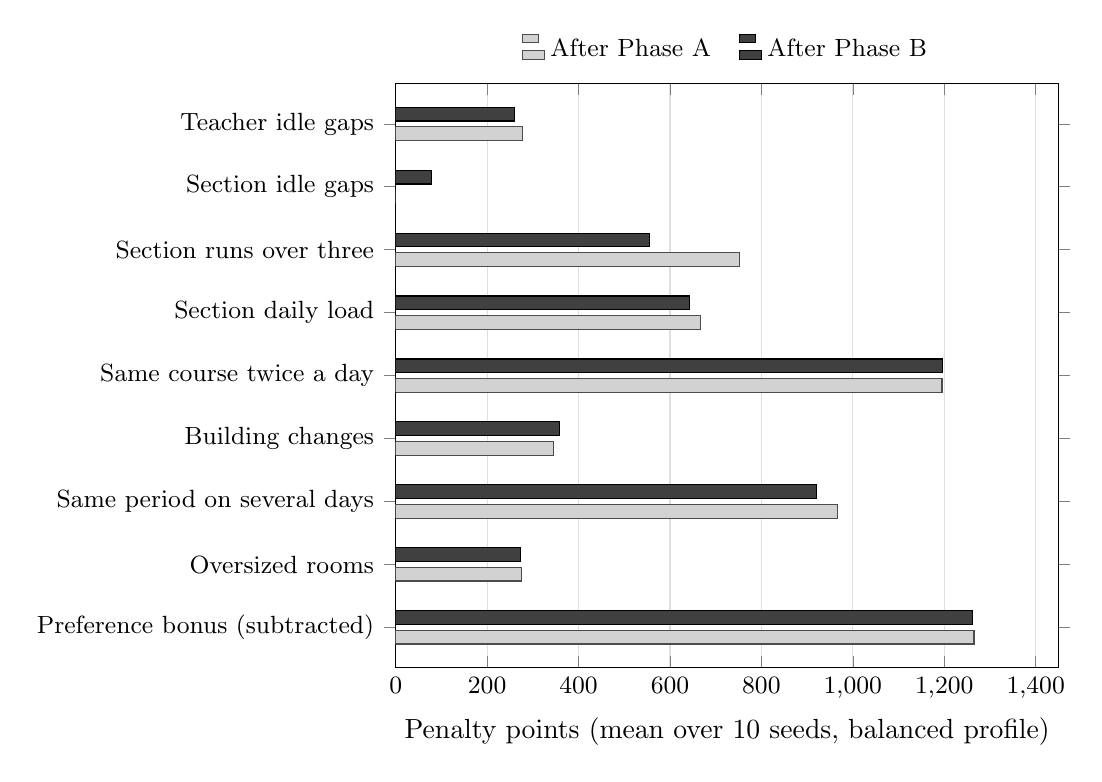
\begin{tikzpicture}
\begin{axis}[
  xbar,
  width=10cm, height=9cm,
  bar width=5pt,
  xmin=0, xmax=1450,
  ytick={1,2,3,4,5,6,7,8,9},
  yticklabels={Teacher idle gaps, Section idle gaps, Section runs over three, Section daily load, Same course twice a day, Building changes, Same period on several days, Oversized rooms, Preference bonus (subtracted)},
  y dir=reverse,
  enlarge y limits=0.08,
  xlabel={Penalty points (mean over 10 seeds, balanced profile)},
  tick label style={font=\small},
  legend style={at={(0.5,1.02)}, anchor=south, legend columns=2, font=\small, draw=none, /tikz/every even column/.append style={column sep=8pt}},
  xmajorgrids, grid style={gray!25},
]
\addplot[fill=gray!35, draw=gray!60!black] coordinates
  {(278,1) (0,2) (752,3) (666,4) (1195,5) (345,6) (966,7) (276,8) (1265,9)};
\addplot[fill=black!75, draw=black] coordinates
  {(260.6,1) (78.8,2) (554.4,3) (642.9,4) (1196.5,5) (357.5,6) (920.7,7) (272.5,8) (1261.2,9)};
\legend{After Phase A, After Phase B}
\end{axis}
\end{tikzpicture}
\caption{Soft-penalty terms before and after simulated annealing (teacher runs over three periods were zero in all runs and are omitted)}
\label{fig:penalty}
\end{figure}

The annealer's gains come almost entirely from breaking up long runs of
consecutive section periods (752 down to 554), partly paid for by new idle
gaps (0 up to 79). The largest term, repeated meetings of a course on one
day, does not move at all. Most of it is structural, as we explain in
Section~\ref{sec:health}.

\subsection{Scaling}

To see how the engine behaves on larger problems we generated a synthetic
family with the same structure as the seeded instance: each section has five
three-hour lecture courses and two laboratory courses taught to two
subgroups in two-hour blocks, with 1.5 lecture halls and 0.95 labs per
section. Table~\ref{tab:scaling} and Figure~\ref{fig:scaling} report the
results; 20 seeds were used up to 32 sections and 10 beyond.

\begin{table}[htbp]
\centering
\small
\begin{tabular}{@{}rrrrrrrr@{}}
\toprule
\textbf{Sections} & \textbf{Session-} & \textbf{Rooms} & \multicolumn{3}{c}{\textbf{Phase A (ms)}} & \textbf{Back-} & \textbf{A+B} \\
\cmidrule(lr){4-6}
 & \textbf{hours} & & \textbf{median} & \textbf{p95} & \textbf{compile} & \textbf{tracks} & \textbf{median (ms)} \\
\midrule
4   & 92    & 10  & 1.08  & 1.89  & 0.57  & 0 & 41.9 \\
8   & 184   & 20  & 0.88  & 1.40  & 0.33  & 0 & 60.5 \\
16  & 368   & 40  & 1.55  & 2.74  & 0.70  & 0 & 145.1 \\
32  & 736   & 79  & 4.32  & 6.67  & 2.61  & 0 & 321.2 \\
64  & 1,472 & 157 & 13.35 & 33.42 & 9.83  & 0 & 588.7 \\
80  & 1,840 & 196 & \multicolumn{5}{l}{stack overflow in 3 of 3 runs} \\
96  & 2,208 & 236 & 29.55 & 47.54 & 21.38 & 0 & 882.6 \\
112 & 2,576 & 275 & \multicolumn{5}{l}{stack overflow in 2 of 2 runs} \\
128 & 2,944 & 314 & \multicolumn{5}{l}{stack overflow in 2 of 3 runs} \\
\bottomrule
\end{tabular}
\caption{Engine time on the synthetic family; every completed run was validated with zero hard violations (at 96 sections, one of three Phase~A+B runs in an earlier measurement overflowed the stack)}
\label{tab:scaling}
\end{table}

\begin{figure}[htbp]
\centering
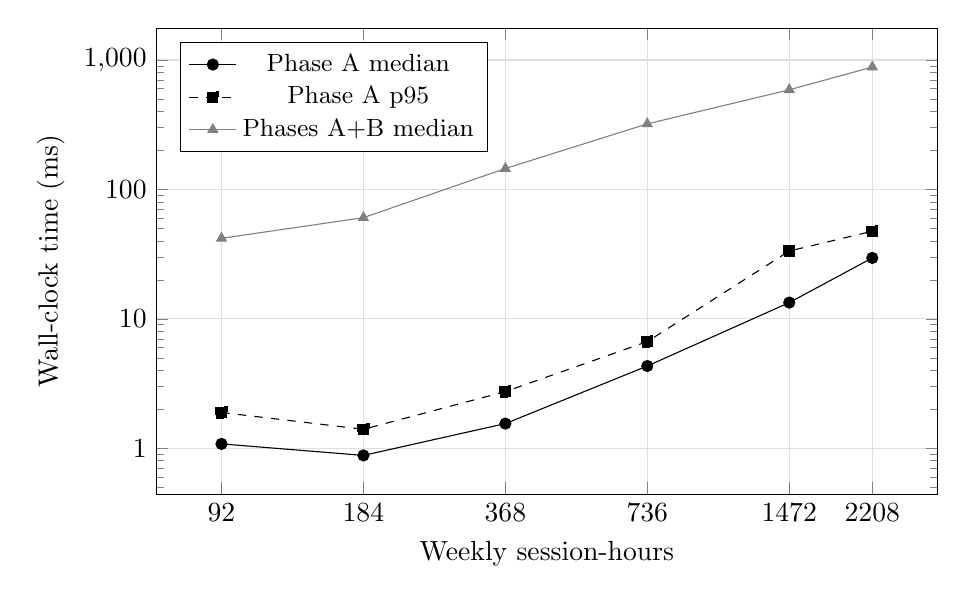
\begin{tikzpicture}
\begin{loglogaxis}[
  width=11.5cm, height=7.5cm,
  xlabel={Weekly session-hours},
  ylabel={Wall-clock time (ms)},
  xtick={92,184,368,736,1472,2208},
  xticklabels={92,184,368,736,1472,2208},
  log ticks with fixed point,
  legend pos=north west,
  legend style={font=\small},
  grid=major, grid style={gray!25},
]
\addplot[black, mark=*] coordinates
  {(92,1.08) (184,0.88) (368,1.55) (736,4.32) (1472,13.35) (2208,29.55)};
\addplot[black, dashed, mark=square*] coordinates
  {(92,1.89) (184,1.40) (368,2.74) (736,6.67) (1472,33.42) (2208,47.54)};
\addplot[gray, mark=triangle*] coordinates
  {(92,41.9) (184,60.5) (368,145.1) (736,321.22) (1472,588.73) (2208,882.57)};
\legend{Phase A median, Phase A p95, Phases A+B median}
\end{loglogaxis}
\end{tikzpicture}
\caption{Engine time against problem size (log--log scale)}
\label{fig:scaling}
\end{figure}

Phase~A stays well under 50\,ms at every size it completes, and at the larger
sizes most of that time is spent in compilation rather than search: 21.4 of
29.6\,ms at 2,208 session-hours. The compiler looks up courses, teachers and
sections with linear scans inside a loop over allocations, and tests block
membership with array searches, so its cost grows faster than linearly.
Phase~B grows roughly in proportion to problem size because every proposal
recomputes the whole penalty from scratch. The overflow rows are discussed in
Section~\ref{sec:stack}.

\subsection{Sensitivity to Room Supply}

The seeded and synthetic instances are generous with lecture rooms. We
fixed the synthetic instance at 32 sections (480 lecture hours a week) and
removed lecture halls one step at a time, with a 3\,s budget per run.
Table~\ref{tab:tight} shows the outcome.

\begin{table}[htbp]
\centering
\small
\begin{tabularx}{\linewidth}{@{}rrYrr@{}}
\toprule
\textbf{Rooms} & \textbf{Utilisation} & \textbf{Outcome} & \textbf{Time (ms)} & \textbf{Backtracks} \\
\midrule
48 & 28.6\% & solved & 5.4 & 0 \\
33 & 41.6\% & solved & 17.3 & 0 \\
32 & 42.9\% & solved & 4.4 & 0 \\
31 & 44.2\% & solved & 25.0 & 0 \\
30 & 45.7\% & no solution within budget & 3,019 & 763,255 \\
28 & 49.0\% & no solution within budget & 3,018 & 883,850 \\
24 & 57.1\% & no solution within budget & 3,023 & 858,596 \\
20 & 68.6\% & no solution within budget & 3,009 & 901,323 \\
16 & 85.7\% & no solution within budget & 3,007 & 939,918 \\
14 & 98.0\% & no solution within budget & 3,003 & 867,381 \\
13 & 105.5\% & no solution, no diagnostic (provably infeasible) & 3,002 & 914,964 \\
\bottomrule
\end{tabularx}
\caption{Phase A as lecture rooms are removed (32 sections, 480 lecture hours, 35 slots; the 33, 31, 30 and 28-room rows come from a follow-up run, which explains the higher times for solved cases)}
\label{tab:tight}
\end{table}

The behaviour is a cliff, not a slope. With 31 rooms the search succeeds
without backtracking; with 30 it gives up after three seconds and three
quarters of a million backtracks, at a room utilisation of only 46\%.
Thirteen rooms offer $13 \times 35 = 455$ room-periods for 480 lecture hours,
so that instance is infeasible by simple counting, yet the system spends its
whole budget searching instead of saying so.

\subsection{Recovery Engine}

We cancelled 100 randomly chosen lectures of the seeded timetable, one at a
time, and ran the recovery search for each. All 100 cancellations received
the full five make-up options. The median search time was 1.5\,ms and the
95th percentile 2.6\,ms. The top-ranked option scored exactly 93 in every
one of the 100 cases, a point we come back to in Section~\ref{sec:minor}.

On the security side, bcrypt at cost 12 took a median of 280\,ms per hash in
the pure-JavaScript implementation used by the project (61\,ms at cost 10),
which is in the range usually recommended for interactive logins.

\subsection{Objectives Against Targets}

Table~\ref{tab:performance} compares each objective from Chapter~1 with the
measured outcome.

\begin{table}[htbp]
\centering
\small
\begin{tabularx}{\linewidth}{@{}P{3.0cm}P{3.0cm}YP{1.8cm}@{}}
\toprule
\textbf{Objective} & \textbf{Target} & \textbf{Achieved} & \textbf{Status} \\
\midrule
O1 Conflict-free generation & 0 hard violations, $< 1$\,s & 0 violations; 7.5\,ms median (Phase~A) & Met \\
O2 Soft optimisation & Measurable reduction, no hard violations & 2.2--5.9\% mean reduction; clash introduced in 19 of 30 runs & Partly met \\
O3 Publication gate & Block every invalid timetable & All 36 clashes flagged; invalid routines unselectable; publish refused with HTTP~422 & Met \\
O4 Recovery & 5 options in $< 50$\,ms & 100 of 100 cancellations; 1.5\,ms median, 2.6\,ms p95 & Met \\
O5 Role-based workflow & 7 roles, lifecycle, audit & Implemented and covered by API tests; no user study yet & Met (not user-tested) \\
O6 Security baseline & Controls in place and tested & 24/24 unit; 53/54 and 18/20 HTTP checks, failures explained above & Met, with test debt \\
\bottomrule
\end{tabularx}
\caption{Project objectives against measured results}
\label{tab:performance}
\end{table}

\section{Analysis}

\subsection{What the Seeded Instance Does and Does Not Tell Us}
\label{sec:seeded}

The headline result, a clash-free timetable for 1,280 students in under
10\,ms, is true, but it would be misleading to stop there. The seeded
instance is easy. It has 50 lecture rooms for 32 sections, no teacher with
more than five hours, and no protected periods. With no availability
restrictions, every allocation has the same 35 feasible slots, so the
fail-first ordering reduces to ``labs first, then lectures'' and carries
little information. Zero backtracks is evidence that the instance is loose,
not that the heuristic is clever. Table~\ref{tab:tight} is the more honest
picture of the search: as soon as rooms are scarcer than sections, it fails
at a modest utilisation.

\subsection{The Annealer's Leaky Feasibility Check}
\label{sec:leak}

Across 30 \textsc{balanced}-mode runs (three profiles, ten seeds), the
validator found 36 hard violations in 19 runs. All 36 had the same code,
\texttt{CROSS\_COHORT\_COLLISION}: a whole-section lecture placed in a slot
where the section's laboratory subgroups were already in session. Phase~A
output never had one. The two routines the server generates by default
(student-focused with seed 1337, faculty-focused with seed 9999) each carried
exactly one such clash, so on the seeded data a coordinator pressing
\emph{Generate} with default settings receives two routines, both marked
invalid, and cannot select either.

The cause is in the annealer's fast check. For a whole-section session it
tests a key that is never written anywhere in the code:

{\small
\begin{verbatim}
if (secWholeOccupancy.has(secKey) ||
    subSecOccupancy.has(`${s.sectionId}_has_sub_${keySlot}`)) return false;
\end{verbatim}
}

Subgroup sessions are recorded under their own subgroup key, so when a
subgroup session comes earlier in the list than a lecture of the same
section at the same slot, the lecture passes the check. The fix is one line:
record a section-level marker whenever a subgroup session is added.
Phase~A does not have the problem because it keeps a per-slot subgroup
counter for every section.

We think this is the most useful result in the report, and not because of the
bug itself. The independent validator caught every one of the 36 clashes,
the selection and publication gates refused to let any of them through, and
the security suite's unexplained HTTP~422 turned out to be the same defect
seen through the API. Had the engine been trusted to report its own hard
violation count, which it hard-codes to zero for every candidate, the clashes
would have reached students.

\subsection{The Health Score Saturates}
\label{sec:health}

The engine's health score was 10, its floor, in every run on the seeded
instance, before and after optimisation. The penalty is an absolute sum, so
on 736 sessions it reaches the thousands and $100 - P$ is deeply negative.
A score that never moves cannot help a coordinator choose between routines.
Part of the penalty is also unavoidable. A two-hour laboratory produces two
session records for the same course on the same day, so the ``same course
twice a day'' term charges for blocks that the hard constraints require, and
charges more when both subgroups of a section have that lab on the same day.
Each of the 64 laboratory course--section pairs therefore contributes at
least 10 points at the balanced weights, 640 in total, which explains why that
term did not move at all under annealing. A
normalised score (penalty per session, or relative to a computed lower
bound) and a distribution term that counts a lab block once would make the
number meaningful.

\subsection{Thrashing Under Scarcity}

The cliff in Table~\ref{tab:tight} has a plausible explanation in the value
ordering. For the first solution every allocation tries slots in the same
order, Monday first period first, so lectures pile into the earliest slots of
the week. While there is at least one lecture room per section, a crowded
slot never runs out of rooms. Below that threshold some allocation deep in
the search finds every slot it wants full, and chronological backtracking
then revisits the most recent decisions, which usually have nothing to do
with the conflict. Our observation that 31 rooms work and 30 do not, with
32 sections of which some are always in labs, is consistent with that
explanation. The standard remedies are well known: randomised or
least-constraining value ordering, conflict-directed backjumping, random
restarts~\cite{russell2021aima}, or a pigeonhole check in Phase~0 so that
the provably infeasible 13-room case is reported in milliseconds.

\subsection{Recursion Depth}
\label{sec:stack}

Phase~A recurses once per placement, so its depth is roughly the number of
session-hours. At 1,840 session-hours it overflowed the default call stack in
every run we made. At 2,208 Phase~A on its own completed in all three runs,
although one of the combined Phase~A and~B runs at that size overflowed. At
2,576 it failed again. The outcome is not monotone in size, which suggests that the stack
frame size depends on whether the just-in-time compiler has optimised the
recursive function by the time the deep calls happen. We did not pin the
mechanism down further. What matters is that the limit exists at about two
and a half times the seeded instance. The project's own design document
targets 12,000 students and around 280 concurrent sessions an hour; at 35
periods a week that is in the order of 9,800 session-hours, well past the
point where we saw failures. The job API runs the engine in a worker thread,
which has a different default stack size, but the synchronous path runs it
on the main thread. Converting the search to an explicit stack removes the
limit entirely.

\subsection{Smaller Issues Found During Review}
\label{sec:minor}

\begin{itemize}
  \item \textbf{Candidate diversity.} The two later candidates are found by
    backtracking from the first solution, so they differ from it only in the
    last allocations of the search order. Even after annealing, 89.5\% to
    98.5\% of session placements were identical between candidates across our
    two measurement runs.
  \item \textbf{Preference indexing.} The preference bonus compares a
    zero-based period index with teachers' preferred periods, which are
    stored as one-based period numbers, so the bonus is awarded to the wrong
    periods.
  \item \textbf{Validator gaps.} The ``one lecture per course per day'' rule
    is hard in Phase~A but only a warning in the validator, and teachers'
    weekly limits are checked by the validator but not during the search.
    Neither caused a failure on our data, but the two components should agree.
  \item \textbf{Our own benchmark script.} The project's solver suite reports
    a ``100\% reduction in search nodes'' against a baseline scheduler. On
    inspection it divides the number of complete candidates found by the
    baseline's count of slot attempts, which are different quantities. On the
    same run the engine made more constraint checks than the baseline (27,318
    against 15,888) and was not faster (4.66 against 4.28\,ms). The same
    script's large-scale section reports results for instances that its
    generator makes infeasible by construction, and its ``property-based''
    section iterates over six fixed sizes and counts an infeasible result as a
    pass. We have not used any of these figures in this report.
  \item \textbf{Comparison solvers.} The DSATUR and greedy solvers behind the
    benchmark view report some quality figures that are fixed constants
    rather than measurements, floor their reported run times at 12\,ms and
    5\,ms, and the greedy solver performs no clash checks at all. The view is
    a useful teaching aid, but its numbers should not be read as evidence.
    An older what-if helper in the recovery library also returns fixed
    projections; the current what-if view no longer uses it and computes its
    figures from the simulated changes.
  \item \textbf{Recovery ranking.} Most scoring factors take one of two or
    three fixed values, so many options tie; the top option scored 93 in all
    100 trials, and the order among tied options falls back to the order of
    the scan (earliest day first).
\end{itemize}

\subsection{Engineering Challenges During Development}

Several of the hardest problems were not algorithmic. Early versions kept
session tokens in browser storage; we moved to \texttt{httpOnly} cookie
sessions so that a script injected into the page cannot read them, which in
turn required the Origin-based CSRF check. Newly registered accounts were at
one point held only in an in-memory map and disappeared on every restart; the
fix was to write them to the users table and to make login wait for the
database to confirm the session write before reporting success. The solver
originally ran inside the request handler and blocked the whole server while
it worked; moving it to a worker thread behind the job API fixed that. The
single-instance persistence design described in Section~\ref{sec:hld} was a deliberate
trade of scalability for simplicity, and we would make the same trade again
at this stage, but it now needs to be revisited.

The most recent change deserves a note of caution. Because the production
deployment had no email provider, verification links were never delivered,
and registration was changed to work without email verification. The
institutional-domain restriction now checks only the text of the address, not
that the registrant controls the mailbox. Self-registered accounts receive
the student role, which limits the exposure to what a student can see and do,
but verification should return once a mail provider is configured. The
project's threat model also notes that the bootstrap endpoint returns the
full academic dataset to every signed-in user, with the portals filtering
what is shown; moving that filtering to the server is on our list.

% ===== CHAPTER 5: CONCLUSION =====

\chapter{Conclusion}
\label{ch:conclusion}

\section{Summary of Work}

We built a working timetabling platform for a multi-department university,
covering master-data setup and import, two-phase timetable generation,
independent validation, review and approval across seven roles, publication
to role-specific portals, and post-publication recovery with make-up
proposals and section polls. The system is a single TypeScript service with
a PostgreSQL store, about 37,000 lines of code, with automated unit, API,
solver and security suites run in continuous integration. Measured against
the objectives set at the start, generation (O1), the publication gate (O3),
recovery (O4), the role-based workflow (O5) and the security baseline (O6)
are met, the last with some test debt. Soft-constraint optimisation (O2) is
only partly met: it improves the penalty slightly but, in its current form,
can break a hard constraint.

\section{Key Findings}

\begin{itemize}
  \item \textbf{Finding 1:} Bitset backtracking with a static fail-first order
    solves the seeded instance (736 session-hours) with no backtracking in
    under 10\,ms, and the validator confirms zero hard violations. The
    instance is loose, however, and the same search fails once lecture rooms
    are fewer than sections.
  \item \textbf{Finding 2:} The independent validator earned its place. It
    caught every one of 36 cross-cohort clashes introduced by the annealer,
    including the clash in each of the two default routines, and the gates
    built on it kept all of them away from students. The underlying defect is
    a one-line error in the annealer's fast check.
  \item \textbf{Finding 3:} Simulated annealing as currently configured buys
    a 2--6\% penalty reduction for roughly 250--300\,ms of extra time, is
    capped by iteration count rather than budget, and is measured by a health
    score that sits at its floor. The optimisation stage needs better
    instrumentation before it can be tuned.
  \item \textbf{Finding 4:} The recursive search overflows the default call
    stack at around 1,800 session-hours, well below the scale the project's
    design documents aim for.
  \item \textbf{Finding 5:} Several of our own early performance claims did
    not survive a careful reading of how they were measured. Defining each
    metric precisely, and checking it against an independent measurement,
    turned out to matter as much as the algorithms themselves.
\end{itemize}

\section{Future Work and Recommendations}
\label{sec:future}

\begin{enumerate}
  \item \textbf{Fixes with immediate effect.} Record a section-level marker
    for subgroup sessions in the annealer's fast check; make the validator and
    Phase~A agree on H9 and H10; correct the preference index; normalise the
    health score; count a laboratory block once in the distribution penalty;
    and update the two test scripts whose expectations predate deliberate
    policy changes.
  \item \textbf{Alternative approaches worth exploring.} Replace chronological
    backtracking with conflict-directed backjumping and randomised restarts,
    add a pigeonhole check on lecture-room capacity to Phase~0, and compare
    the annealer against late-acceptance hill climbing~\cite{burke2017late}
    and tabu search~\cite{lu2010adaptive} with incremental (delta) penalty
    evaluation. For recovery after long absences, formulate the minimal
    perturbation problem as an integer program~\cite{phillips2017integer}.
  \item \textbf{Scalability improvements.} Make the search iterative so that
    depth is no longer bounded by the call stack; index the compiler's
    lookups; store entities as rows rather than one JSON document so that more
    than one instance can serve traffic; and move rate-limit counters and
    solver jobs out of process memory.
  \item \textbf{Integration with other systems.} Export instances in the
    curriculum-based ITC format~\cite{bonutti2012benchmarking} so that the
    engine can be compared with published results, and connect enrolment and
    room-booking data from the institute's existing systems instead of
    relying only on the workbook import.
  \item \textbf{Real-world deployment considerations.} Restore email
    verification once a mail provider is configured; filter the bootstrap
    payload by role on the server; reconsider whether the person who
    generates a timetable should also be able to publish it without a second
    approval; and run a usability study with two or three coordinators and a
    sample of faculty and students before the next timetable cycle.
\end{enumerate}

\section{Final Remarks}

When we started, we thought the hard part of this project would be the
search algorithm. It was not. The search was the part that worked first.
What took most of our time was everything around it: getting sessions,
persistence and permissions right, deciding what a ``good'' timetable means
in numbers, and, towards the end, learning to distrust our own measurements
until we had checked them a second way. If there is one design decision we
would defend to the next team that works on this code, it is the separation
between the component that builds a timetable and the component that judges
it. Every serious defect we found in the engine was found because that
separation existed.

% ===== BIBLIOGRAPHY =====

% Print bibliography with heading in TOC
\printbibliography[heading=bibintoc]

% ===== APPENDIX =====

\appendix

\chapter{Reproducing the Measurements}
\label{app:repro}

All results in Chapter~\ref{ch:results} can be reproduced from the public
repository~\cite{intellischedule2026repo} at commit \texttt{cfca8da}.

\paragraph{Project suites.} After \texttt{npm install}:
{\small
\begin{verbatim}
npx tsc --noEmit          # type check
npm test                  # unit tests + end-to-end API audit
npm run test:solver       # project solver suite
npm run test:security     # needs the server on port 3000
\end{verbatim}
}
The security suite expects a server started with the same environment as
the CI workflow:
{\small
\begin{verbatim}
NODE_ENV=test
ALLOW_TEST_RESET_TOKEN=true
PUBLIC_DEMO_ENABLED=true
SEED_USER_PASSWORD=<a test password>
DEMO_ACCOUNT_PASSWORD=<a test password>
\end{verbatim}
}

\paragraph{Our measurement harness.} The harness (\texttt{bench.mts}) and
the raw logs are supplied with this report. It imports the engine, validator
and recovery modules from the repository without modification. Copied into
the repository's \texttt{scripts} folder, it is run from the repository
root with:
\begin{verbatim}
node --import tsx scripts/bench.mts results.json
\end{verbatim}
It runs, in order: dataset statistics; Phase~A and Phase~B on the seeded
instance (three profiles, ten seeds each, seeds $101, 108, \dots, 164$);
classification of validator violations; the two default routines;
candidate diversity; the synthetic scaling family; the room-scarcity sweep;
100 random cancellations through the recovery search; and bcrypt timings.
Penalties and violation counts are deterministic for a given seed as long as
Phase~B completes its 300 proposals within the budget. Timings vary between
runs and machines by up to a factor of two at the 95th percentile in our
experience; medians are more stable.

\end{document}
